\chapter{Demonstration}

\section{Video steganography sử dụng LSB}

Trong phần này, chúng tôi sử dụng LSB để ẩn video trong video trong miền không gian.

Yêu cầu video bí mật phải ngắn hơn video bìa. Trong ví dụ này, phần âm thanh cũng được chung tôi sử dụng LSB để mã hóa. Chúng tôi sử dụng 4 bit cuối ít quan trọng nhất của video bìa và thay vào đó là 4 bit của video bí mật. Thư viện ffmpeg được chúng tôi xử dụng để xử lý ảnh. Video sẽ được chúng tôi xử lý thành các khung ảnh nhỏ hơn và xử lý tuần tự.

\begin{figure*}[!h]
    \centering
    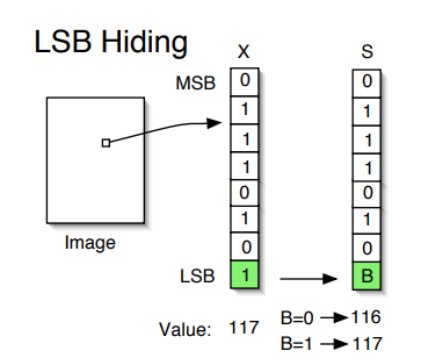
\includegraphics[width=0.6\textwidth]{graphics/chapter-3/lsb_hiding.PNG}
    \caption{Hình minh họa cho LSB}
    \label{fig:LSB}
\end{figure*}

\section{Video steganography trong thủy vân (watermarking)}

Trong phần này, chúng tôi trình bày 1 công cụ ẩn thông tin bao gồm 4 phương pháp để ẩn thông tin được biểu diễn chi tiết ở Hình \ref{tab:demo2_algo} trong miền biến đổi. 

\begin{figure}
    \centering
    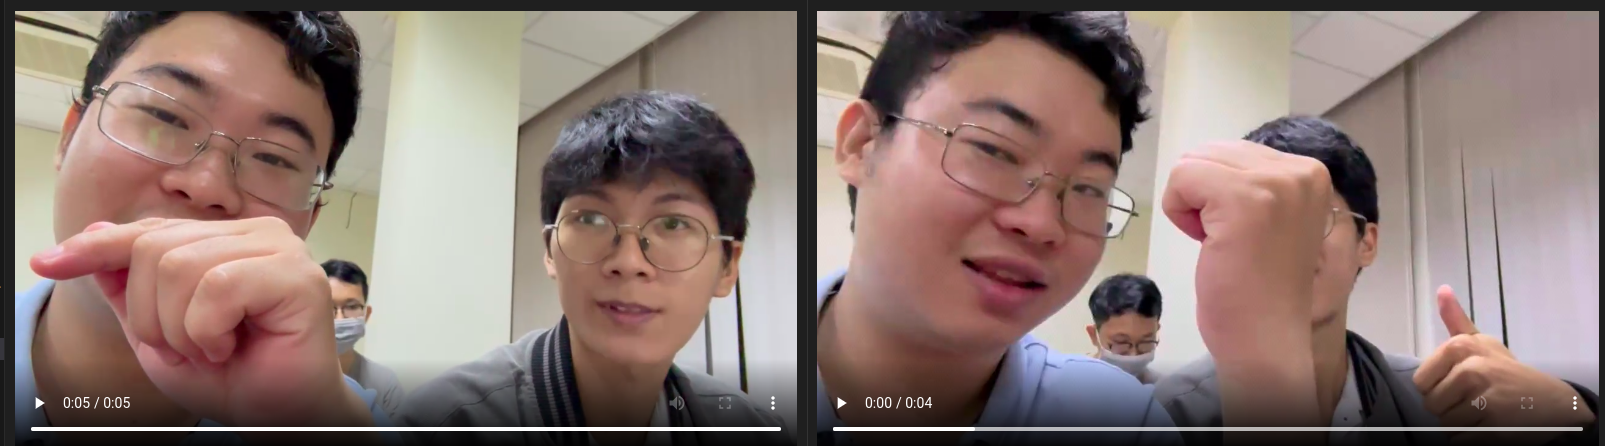
\includegraphics[scale=0.4]{graphics/chapter-3/chap3-video-hiding-video.png}
    \caption{Video trước (trái) và sau khi đã nhúng watermark}
    \label{fig:chap3-video-hiding-video}
\end{figure}


\begin{figure}
    \centering
    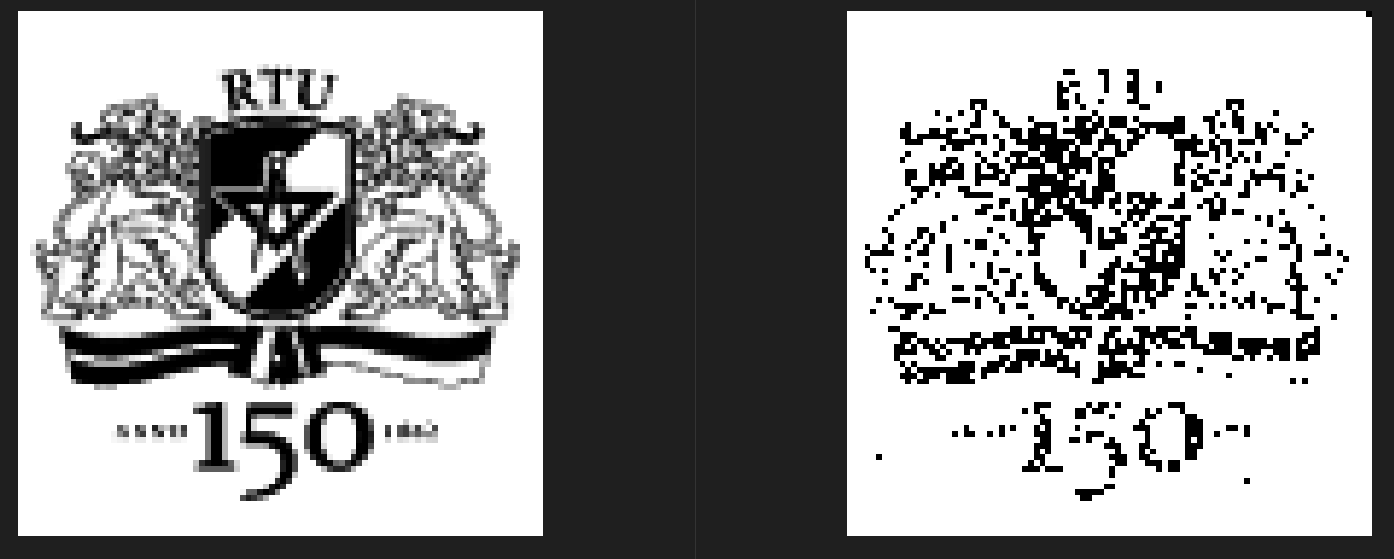
\includegraphics[scale=0.4]{graphics/chapter-3/chap3-result-water-mark.png}
    \caption{Hình ảnh watermark sau khi trích xuất từ video (phải) và trước khi nhúng}
    \label{fig:chap3-result-water-mark}
\end{figure}

Công cụ này dựa trên thư viện Xuggler và được viết bằng Java để hỗ trợ đa nền tảng. Các thử nghiệm đã được thực hiện bằng cách nhúng vào các tệp định dạng .mp4 với codec H.264 và MPEG4 (phần mềm hỗ trợ tất cả các định dạng và codec được Xuggler hỗ trợ, tuy nhiên một số không phù hợp để nhúng).

\begin{table}[ht]
    \centering
    \caption{Bốn thuật toán sử dụng trong demo}
    \label{tab:demo2_algo}
    \begin{tabular}{| p{.25\textwidth} | p{.70\textwidth} |}
        \hline
        \textbf{Phương pháp} & \textbf{Mô tả}  \\
        \hline
        DCT \cite{algo1_kaur2011steganographic} & Phương pháp dựa trên việc nhúng dữ liệu vào các hệ số DCT 8 x 8 của một khung trong kênh Y của không gian màu YCbCr. Hai hệ số đã được chọn và so sánh – tùy thuộc vào hệ số nào có giá trị lớn hơn, giá trị 1 hoặc 0 được giải   mã. \\
        \hline
        DCT \cite{algo2_kothari2011performance} & Phương pháp tương tự như phương pháp DCT ở trên, nhưng sử dụng các hệ số khác nhau và hoạt động trên kênh G của không gian màu RGB. \\
        \hline
        DCT \cite{algo3_al2012robust} & Phương pháp dựa trên việc nhúng dữ liệu vào các hệ số khối 8 x 8 DCT bằng  cách sử dụng lượng tử hóa ghép nối và không ghép nối. Kênh G của không gian  màu RGB đã được sử dụng cho các thử nghiệm. $\delta$ cho thấy độ chính xác của lượng tử hóa. \\ 
        \hline
        DWT \cite{algo4_chetan2010dwt} & Phương pháp nhúng vào các vùng LL, HH và HL của phép biến đổi DWT. Kênh Y của không gian màu YCbCr được sử dụng trong phương pháp. \\
        \hline
    \end{tabular}
\end{table}

% \begin{table}[!h]
% \centering
% \caption{4 thuật toán sử dụng trong demo} 
% \label{tab:demo2_algo}
% \resizebox{\textwidth}{!}{
% \begin{tabular}{|c|c|}
% \hline
% \textbf{Phương pháp} &
%   \textbf{Mô tả} \\ \hline
% DCT \cite{algo1_kaur2011steganographic} &
%   \begin{tabular}[c]{@{}c@{}}Phương pháp dựa trên việc nhúng dữ liệu vào các hệ số DCT 8 x 8 của một \\ khung trong kênh Y của không gian màu YCbCr. Hai hệ số đã được chọn và so \\ sánh – tùy thuộc vào hệ số nào có giá trị lớn hơn, giá trị 1 hoặc 0 được giải   mã.\end{tabular} \\ \hline
% DCT \cite{algo2_kothari2011performance} &
%   \begin{tabular}[c]{@{}c@{}}Phương pháp tương tự như phương pháp DCT ở trên, nhưng sử dụng các hệ số\\  khác nhau và hoạt động trên kênh G của không gian màu RGB.\end{tabular} \\ \hline
% DCT \cite{algo3_al2012robust} &
%   \begin{tabular}[c]{@{}c@{}}Phương pháp dựa trên việc nhúng dữ liệu vào các hệ số khối 8 x 8 DCT bằng \\ cách sử dụng lượng tử hóa ghép nối và không ghép nối. Kênh G của không gian\\  màu RGB đã được sử dụng cho các thử nghiệm. Δ cho thấy độ chính xác của lượng   tử hóa.\end{tabular} \\ \hline
% DWT \cite{algo4_chetan2010dwt} &
%   \begin{tabular}[c]{@{}c@{}}Phương pháp nhúng vào các vùng LL, HH và HL của phép biến đổi DWT. Kênh Y \\ của không gian màu YCbCr được sử dụng trong phương pháp.\end{tabular} \\ \hline
% \end{tabular}
% }
% \end{table}

Trong nỗ lực không ngừng để tối ưu hóa việc ẩn giấu thông tin trong hình ảnh và video, chúng tôi đã sử dụng các thuật toán tiên tiến, chủ yếu dựa trên phương pháp biến tướng của Discrete Cosine Transforms (DCT) và Discrete Wavelet Transforms (DWT). Nhờ sự điều chỉnh tinh vi các hệ số và kênh màu (RGB hoặc YCbCr), chúng tôi đã xây dựng được một cơ chế mạnh mẽ để thực hiện việc ẩn các video vào các video khác.

Các hệ thống mã hóa thông tin đang dần trở nên thông minh hơn, và một phần quan trọng của điều này là việc thay đổi cách thông tin được biểu diễn trên hình ảnh. Hai loại kênh màu chính - RGB và YCbCr - đã chứng tỏ khả năng linh hoạt trong việc chuyển đổi giữa chúng thông qua những dòng mã lệnh được thiết kế cẩn thận. Điều này làm cho việc tạo ra hình ảnh và video mới kết hợp thông tin bí mật trở nên dễ dàng và hiệu quả hơn.

Mô hình màu RGB (Red Green Blue) là mô hình cơ bản dựa trên việc kết hợp ba màu cơ bản: đỏ, xanh lá cây và xanh dương. Mỗi pixel trong hình ảnh được biểu diễn bằng cách chỉ định giá trị của ba kênh màu này. Mô hình RGB phản ánh cách con người cảm nhận màu sắc thông qua ba màu cơ bản này. Mặc dù dễ dàng hiểu và có thể biểu diễn trực tiếp các màu sắc cơ bản, tuy nhiên, mô hình này không phản ánh một cách chính xác khả năng nhận biết màu sắc của mắt người. Thường không thích hợp cho việc xử lý và nén hình ảnh.

Trái với đó, mô hình màu YCbCr (Luminance Chrominance) chia thành ba kênh: Y biểu diễn thông tin về độ sáng của điểm ảnh, trong khi Cb và Cr biểu diễn thông tin về màu sắc. Mô hình YCbCr thể hiện tốt hơn khả năng nhận biết màu sắc của mắt người, điều này khiến nó phù hợp cho việc xử lý hình ảnh, nén và truyền tải qua các kênh có băng thông hạn chế. Tính chất này đặc biệt hữu ích khi cần tách biệt thông tin độ sáng và thông tin màu sắc để thực hiện các phép biến đổi hoặc giảm dung lượng dữ liệu.

Mặc dù YCbCr có nhiều ưu điểm trong việc xử lý hình ảnh, việc chuyển đổi giữa RGB và YCbCr vẫn cần thiết khi cần hiển thị trực tiếp trên các thiết bị RGB. Nhưng với khả năng tách biệt thông tin màu sắc và độ sáng, YCbCr vẫn là một lựa chọn phổ biến trong việc xử lý hình ảnh và video để đảm bảo chất lượng và khả năng nhận biết màu sắc tốt hơn.

Discrete Cosine Transforms (DCT) là một phương pháp biến đổi tín hiệu từ miền thời gian sang miền tần số. Đặc biệt, DCT chia tín hiệu thành các khung nhỏ, sau đó biến đổi mỗi khung bằng cách tính tổ hợp tuyến tính của các hàm cosin với các tần số khác nhau. Kết quả là một tập hệ số DCT thể hiện mức độ xuất hiện của các tần số trong từng khung. DCT thường được áp dụng rộng rãi trong nhiều lĩnh vực như nén hình ảnh (ví dụ: định dạng JPEG) và nén âm thanh (ví dụ: định dạng MP3). Hơn nữa, DCT còn được áp dụng trong việc ẩn thông tin, khi thông tin bí mật được nhúng vào các hệ số tần số thấp, mà mắt người ít nhạy cảm.

Tổng cộng, việc sử dụng các phương pháp biến đổi như DCT và tận dụng các mô hình biểu diễn màu sắc như RGB và YCbCr đã đóng một vai trò quan trọng trong việc tối ưu hóa quá trình ẩn thông tin và xử lý hình ảnh. Việc lựa chọn kỹ thuật phù hợp sẽ phụ thuộc vào mục tiêu cụ thể của ứng dụng và yêu cầu về chất lượng.


\begin{figure*}[!h]
    \centering
    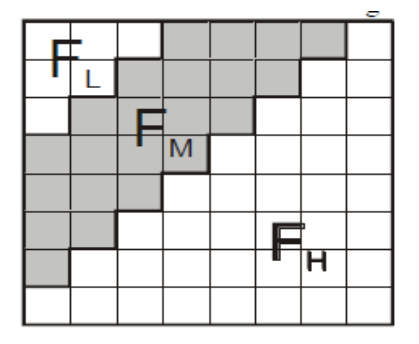
\includegraphics[width=0.6\textwidth]{graphics/chapter-3/DCT_algo1.PNG}
    \caption{Hình minh họa cho DCT}
    \label{fig:PNG}
\end{figure*}

DWT là một phương pháp biến đổi tín hiệu thành các thành phần sóng con ở các tần số và độ phân giải khác nhau. Thay vì sử dụng các hàm cosin như DCT, DWT thực hiện biến đổi bằng cách sử dụng các bộ lọc sóng con. Tín hiệu được phân tách thành các thành phần sóng con ở các tần số thấp và cao, cùng với các mức độ phân giải khác nhau. DWT thường được sử dụng trong nhiều ứng dụng như nén hình ảnh (Wavelet-based image compression) và phân tích tín hiệu y tế. Cũng như DCT, DWT có khả năng ẩn thông tin bằng cách chèn dữ liệu vào các thành phần sóng con thấp tần số hoặc thấp độ phân giải.

\begin{figure*}[!h]
    \centering
    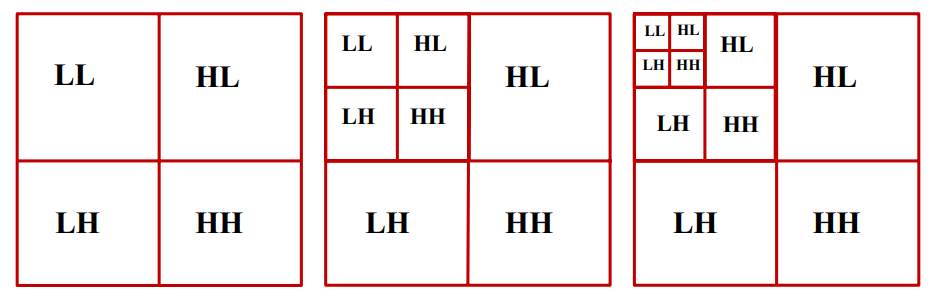
\includegraphics[width=0.6\textwidth]{graphics/chapter-3/DWT.PNG}
    \caption{Hình minh họa cho DWT}
    \label{fig:PNG}
\end{figure*}


\section{Video steganography sử dụng học máy}
Trong phần này, chúng tôi chứng tỏ sự tinh vi và đột phá của một mạng thần kinh tích chập tiên tiến, thường được gọi là convolutional neural network, nhằm mục đích tối ưu hóa việc ẩn những video trong video. Nhiệm vụ đặc biệt quan trọng mà chúng tôi đã đặt ra là ẩn đi một hình ảnh màu có kích thước to lớn (N*N RGB) vào trong một bức tranh khác cùng kích thước. Qua quá trình đào tạo mạng lưới neural sâu song song, chúng tôi đã xây dựng một cặp quy trình quan trọng: quá trình mã hóa và quá trình giải mã, hai khía cạnh này hoạt động như một đôi hoàn thiện nhau. Tại cốt lõi của kỹ thuật này là khả năng nén hình ảnh thông qua việc sử dụng các mạng mã hóa tự động (auto-encoding networks). Toàn bộ hệ thống đã được đào tạo để "học" cách chuyển đổi thông tin từ hình ảnh bí mật vào những phần ít được chú ý nhất trong hình ảnh chứa, và sau đó "học" cách khôi phục và tái tạo thông tin tương tự từ hình ảnh chứa này. Mục tiêu là thực hiện việc mã hóa thông tin một cách hiệu quả, đồng thời giảm thiểu tổn thất dữ liệu.

Chúng tôi đã thực hiện quá trình đào tạo một bộ cặp mạng ẩn và hiển thị đồng thời, sử dụng mô hình bộ mã hóa tự động và sử dụng thư viện Keras để hỗ trợ cho quá trình này. Mô hình này bao gồm hai lớp đầu vào, mỗi lớp tương ứng với một cặp hình ảnh gồm hình ảnh bí mật và hình ảnh bao quanh, và có hai lớp đầu ra tương ứng với đầu vào của chúng. Do mô hình dựa trên kiến trúc mã hóa tự động, việc gán nhãn trong quá trình đào tạo phải tương ứng với đầu vào của nó.

Kiến trúc mạng neural của chúng tôi bao gồm ba phần cốt lõi: Phần Chuẩn bị (Prepare block), Phần Ẩn (Hide block) và Phần Tiết lộ (Reveal block). Trong phần Chuẩn bị, chúng tôi đã thực hiện việc biến đổi các điểm ảnh màu ban đầu thành những đặc trưng có ý nghĩa cao hơn, giúp việc mã hóa hình ảnh trở nên dễ dàng và hiệu quả hơn. Tiếp theo, chúng tôi đã tiến hành việc ẩn hình ảnh đã được biến đổi vào trong hình ảnh bao quanh thông qua sự áp dụng của Phần Ẩn, tạo ra một hình ảnh vùng chứa (container image) đặc biệt. Cuối cùng, trong Phần Tiết lộ, chúng tôi đã thực hiện việc giải mã hình ảnh vùng chứa để tạo ra đầu ra bí mật ban đầu, đảm bảo rằng thông tin quý báu được khôi phục một cách chính xác. Do đó, biểu đồ huấn luyện ở hình \ref{fig:train_graph} có hai đầu vào và hai đầu ra.

\begin{figure*}[!h]
    \centering
    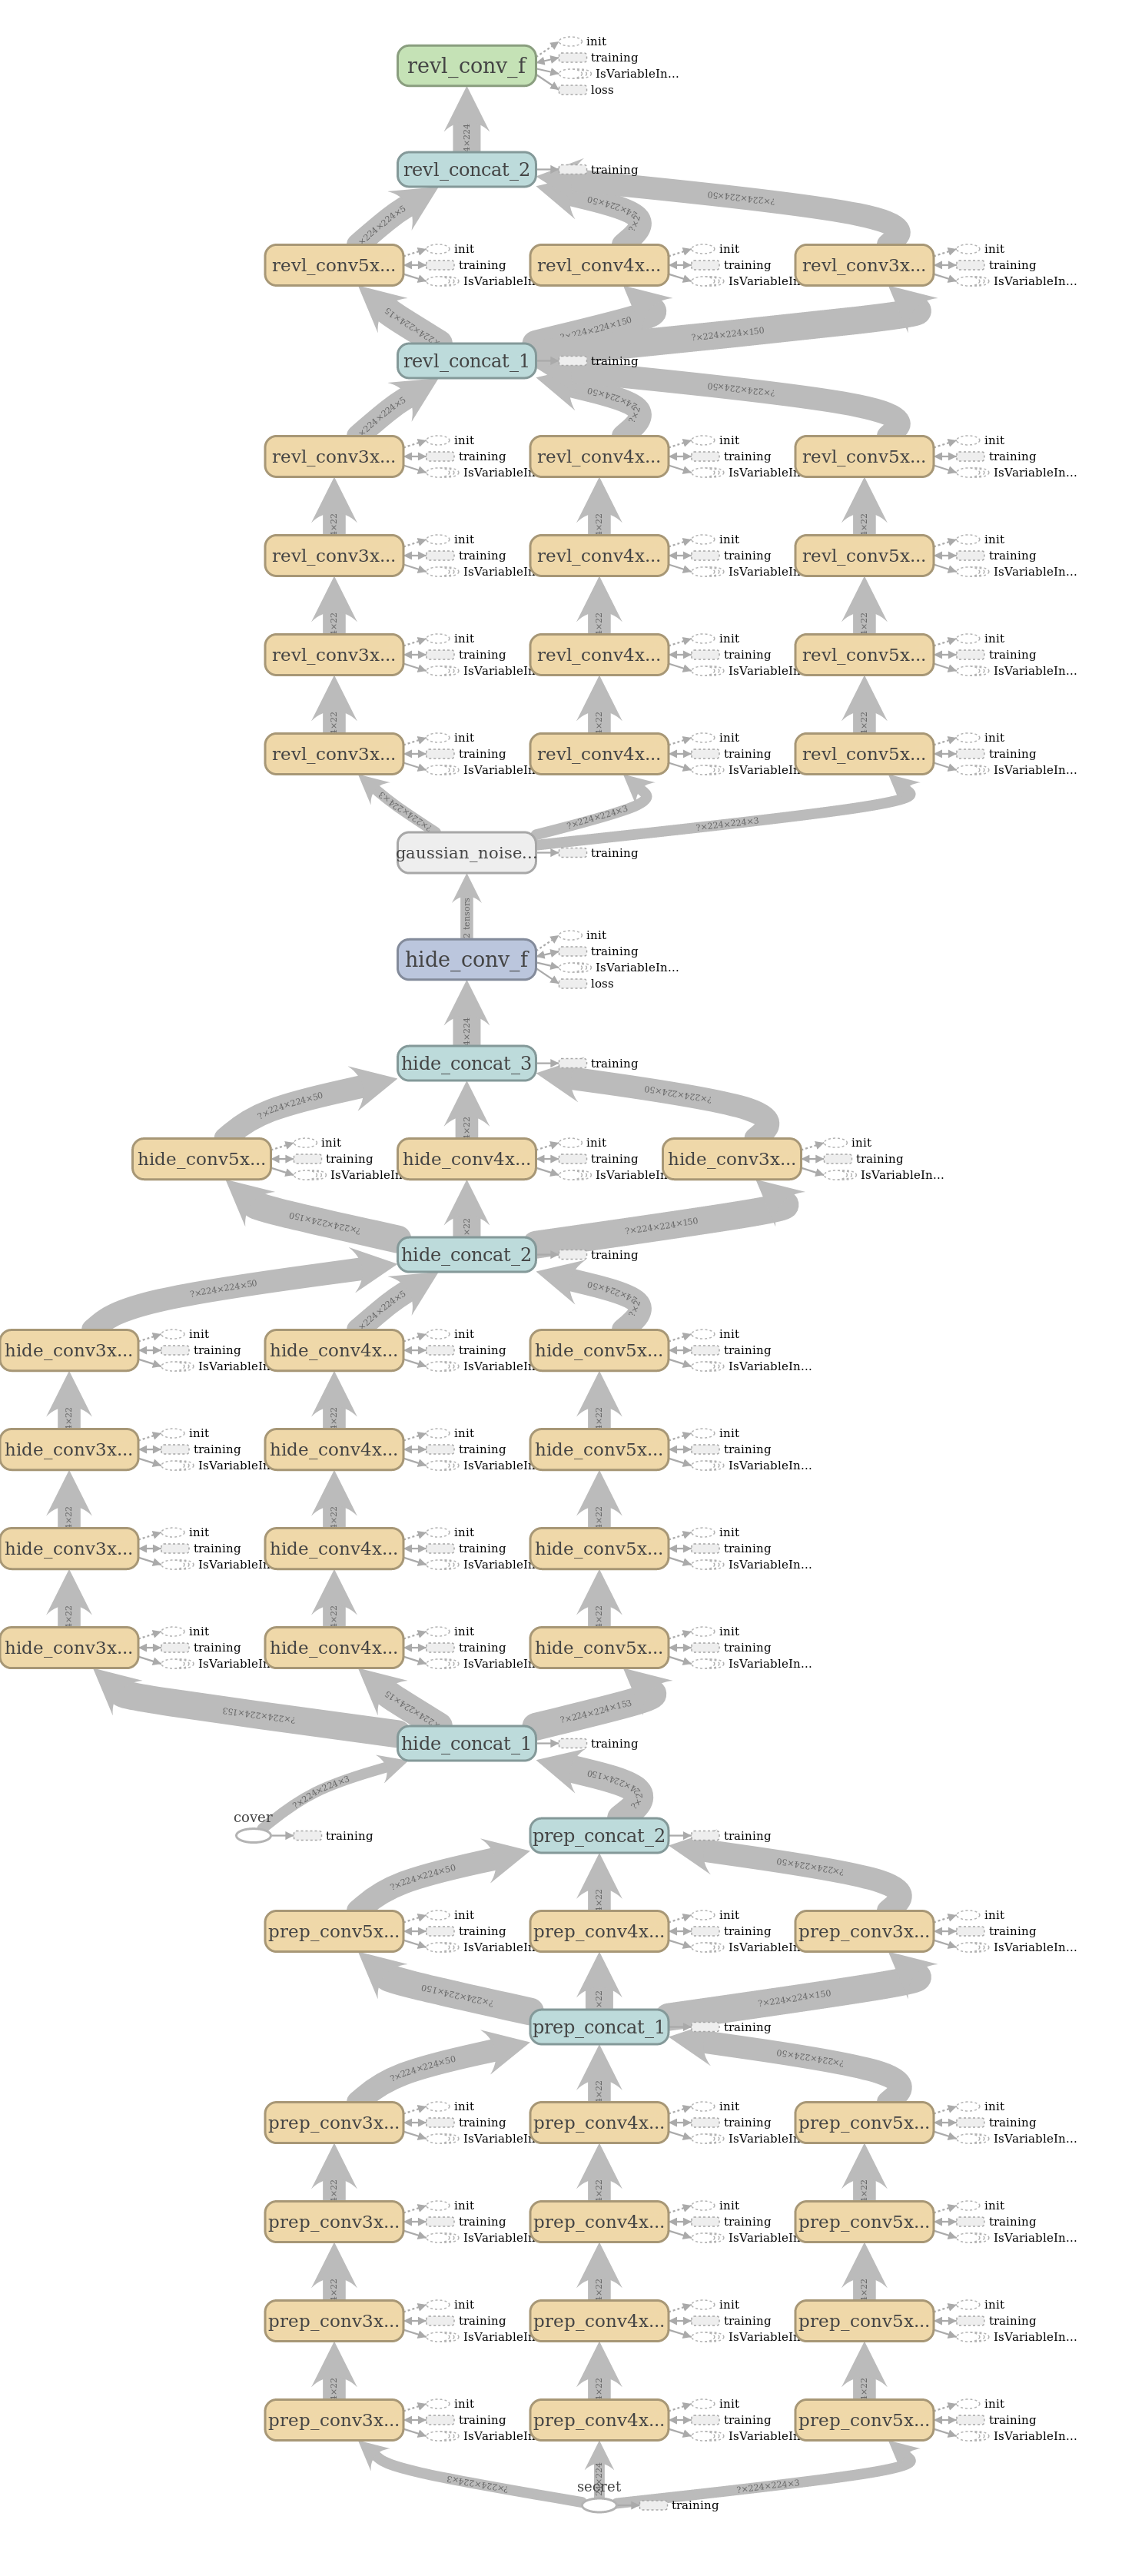
\includegraphics[width=0.6\textwidth]{graphics/chapter-3/train_graph.png}
    \caption{Biểu đồ huấn luyện của mô hình mạng tích chập}
    \label{fig:train_graph}
\end{figure*}


Chúng tôi sử dụng hàm \textbf{weighted L2 loss} và \textbf{Adam optimizer} để huấn luyện mô hình.

Để đảm bảo rằng các mạng không chỉ mã hóa hình ảnh bí mật trong LSB, một lượng nhiễu nhỏ được thêm vào đầu ra của mạng thứ hai (ví dụ: vào hình ảnh vùng chứa được tạo) trong quá trình đào tạo.

Sau khi đào tạo, chúng tôi chia mô hình được đào tạo thành hai: mạng mã hóa và mạng giải mã (chúng tôi loại bỏ lớp nhiễu). Mạng ẩn có hai đầu vào tương ứng với ảnh bí mật và ảnh bìa và một đầu ra tương ứng với ảnh vùng chứa (container image). Mạng giải mã lấy hình ảnh vùng chứa làm đầu vào và tiết lộ (giải mã) hình ảnh bí mật làm đầu ra.

Mạng giải mã được sử dụng bởi người gửi; trong khi mạng mã hóa được dùng bởi người nhận. Người nhận chỉ có quyền truy cập vào hình ảnh vùng chứa. 

Trong video, video sẽ được tách thành các frame nhỏ và mô hình sẽ xử lý 4 frame 1 lần.


\begin{figure}
    \centering
    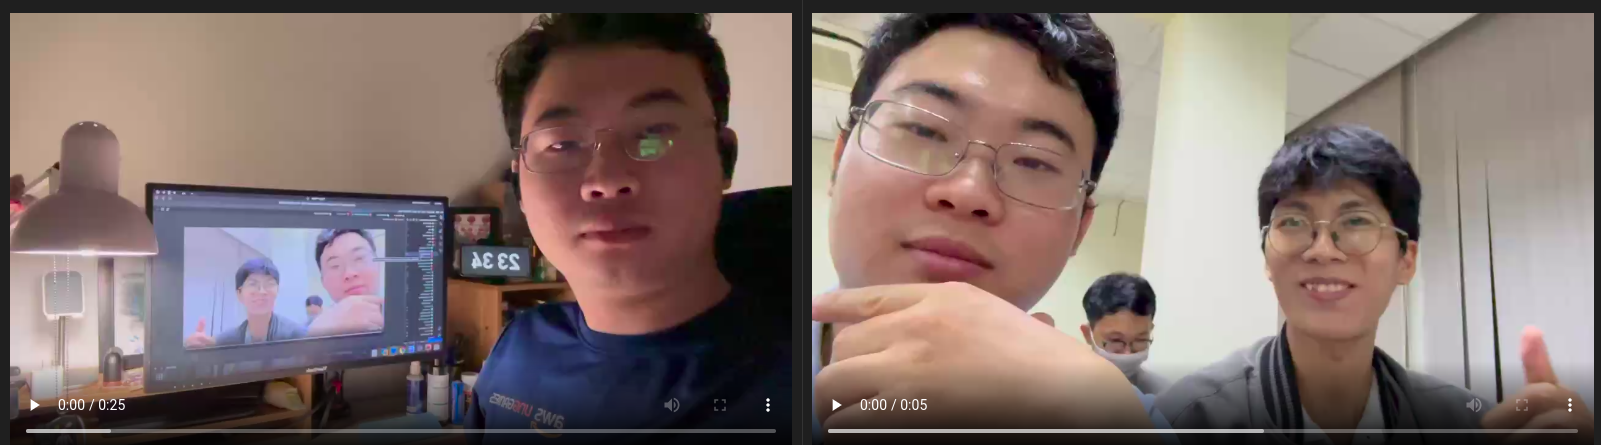
\includegraphics[scale=0.4]{graphics/chapter-3/chap3-video-hiding-to-video.png}
    \caption{Cover video (trái) và video secret muốn ẩn vào trong cover}
    \label{fig:chap3-video-hiding-to-video}
\end{figure}

\begin{figure}
    \centering
    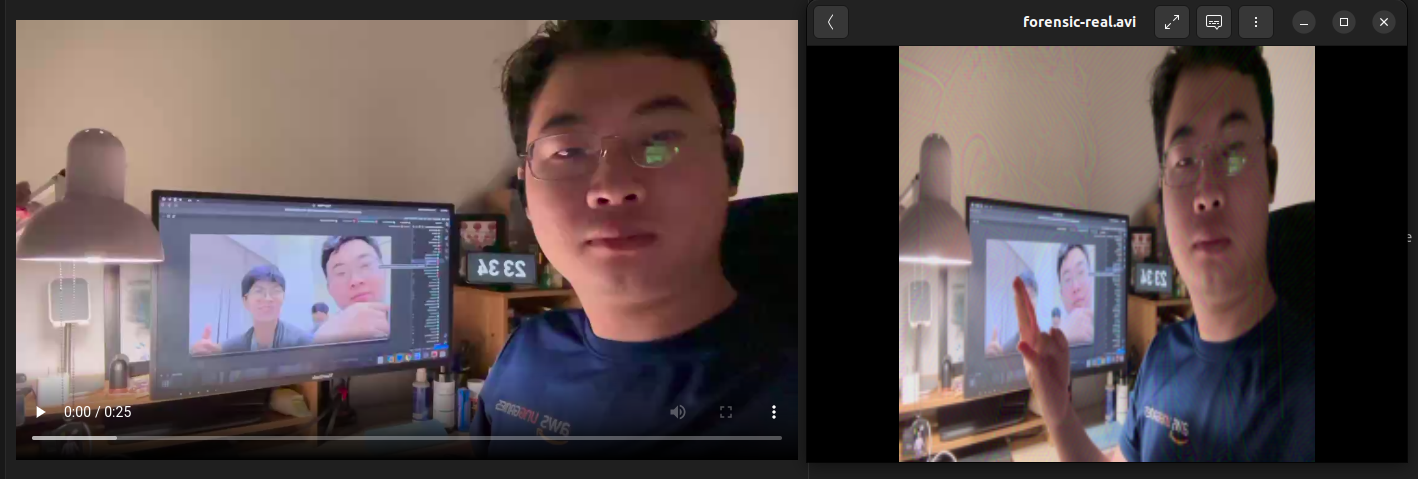
\includegraphics[scale=0.4]{graphics/chapter-3/chap3-video-after-hiding.png}
    \caption{Video trước (trái) và sau khi đã nhúng một video khác vào}
    \label{fig:enter-label}
\end{figure}